\documentclass[a4paper, amsfonts, amssymb, amsmath, reprint, showkeys, nofootinbib, twoside]{revtex4-1}
\usepackage[english]{babel}
\usepackage[utf8]{inputenc}
\usepackage[colorinlistoftodos, color=green!40, prependcaption]{todonotes}
\usepackage{amsthm}
\usepackage{mathtools}
\usepackage{physics}
\usepackage{xcolor}
\usepackage{graphicx}
\usepackage{subfig}
\usepackage[left=23mm,right=13mm,top=35mm,columnsep=15pt]{geometry} 
\usepackage{adjustbox}
\usepackage{placeins}
\usepackage[T1]{fontenc}
\usepackage{lipsum}
\usepackage{csquotes}
\usepackage[pdftex, pdftitle={Article}, pdfauthor={Author}]{hyperref} % For hyperlinks in the PDF
%\setlength{\marginparwidth}{2.5cm}
\bibliographystyle{apsrev4-1}
\begin{document}
\title{When one door's closing... open another?}

\author{Robert Hart}
    \email[Correspondence email address: ]{rhart1@mail.usf.edu}% Your name
    \affiliation{University of South Florida, Department of Physics, Tampa, FL, USA}
    \affiliation{University of South Florida, Department of Mathematics and Statistics, Tampa, FL, USA}
\author{Sierra LaRosa}
    \email[Correspondence email address: ]{sierralarosa@mail.usf.edu}
    \affiliation{University of South Florida, Department of Physics, Tampa, FL, USA}
\author{Zihe Ye}
    \email[Correspondence email address: ]{ziheye@mail.usf.edu }
    \affiliation{University of South Florida, Department of Computer Science and Engineering, Tampa, FL, USA}
    \affiliation{University of South Florida, Department of Physics, Tampa, FL, USA}
    \affiliation{University of South Florida, Department of Mathematics and Statistics, Tampa, FL, USA}







\date{\today} % Leave empty to omit a date

\begin{abstract}
Here we consider a problem which occurs in everyday life, relating to the challenges of our current situation in that here in Spring 2020, we would like to remain distant from one another to keep from the spread of COVID-19. We develop a number of mathematical formalisms for tackling the problem and allow for a number of specific cases in which they apply. We further model computationally our developments under ideal conditions, and then show that they are consistent with experiment. And lastly, we answer the question posed in the title.
\end{abstract}

\keywords{Mechanics, Damping Effects, Experiment}


\maketitle

\section{Introduction} \label{sec:Introduction}
    Say you are walking behind someone at some distance, and the two of you come to a set of double doors. The person in front of you opens one of the doors, but is rather busy and opts not to hold the door for you. As you approach the doors, the open door is now swinging back towards you. Should you take the open, swinging door, or should you take the closed door?

    Obviously, if you can just slip through (if the person in front of you has left the door rather widely open), then you should take the open door. However if the open door is nearly closed, the angular momentum of the door will (likely) be at its greatest value. In this case, not only will you need to push the open door (nearly) as far as you would the closed door, but you would also need to account for the additional angular impulse required to change the direction of the angular momentum, and thus you should take the closed door. 

    In this paper we will discuss the work required to open the closed door versus different cases of the closing door, and develop a model based on such. Further, we will do experiment as well as a number of numerical/computational analyses.  %I believe leaving the sections in separate files is more organized, change it if you desire 
\begin{figure}[htp]
\centering
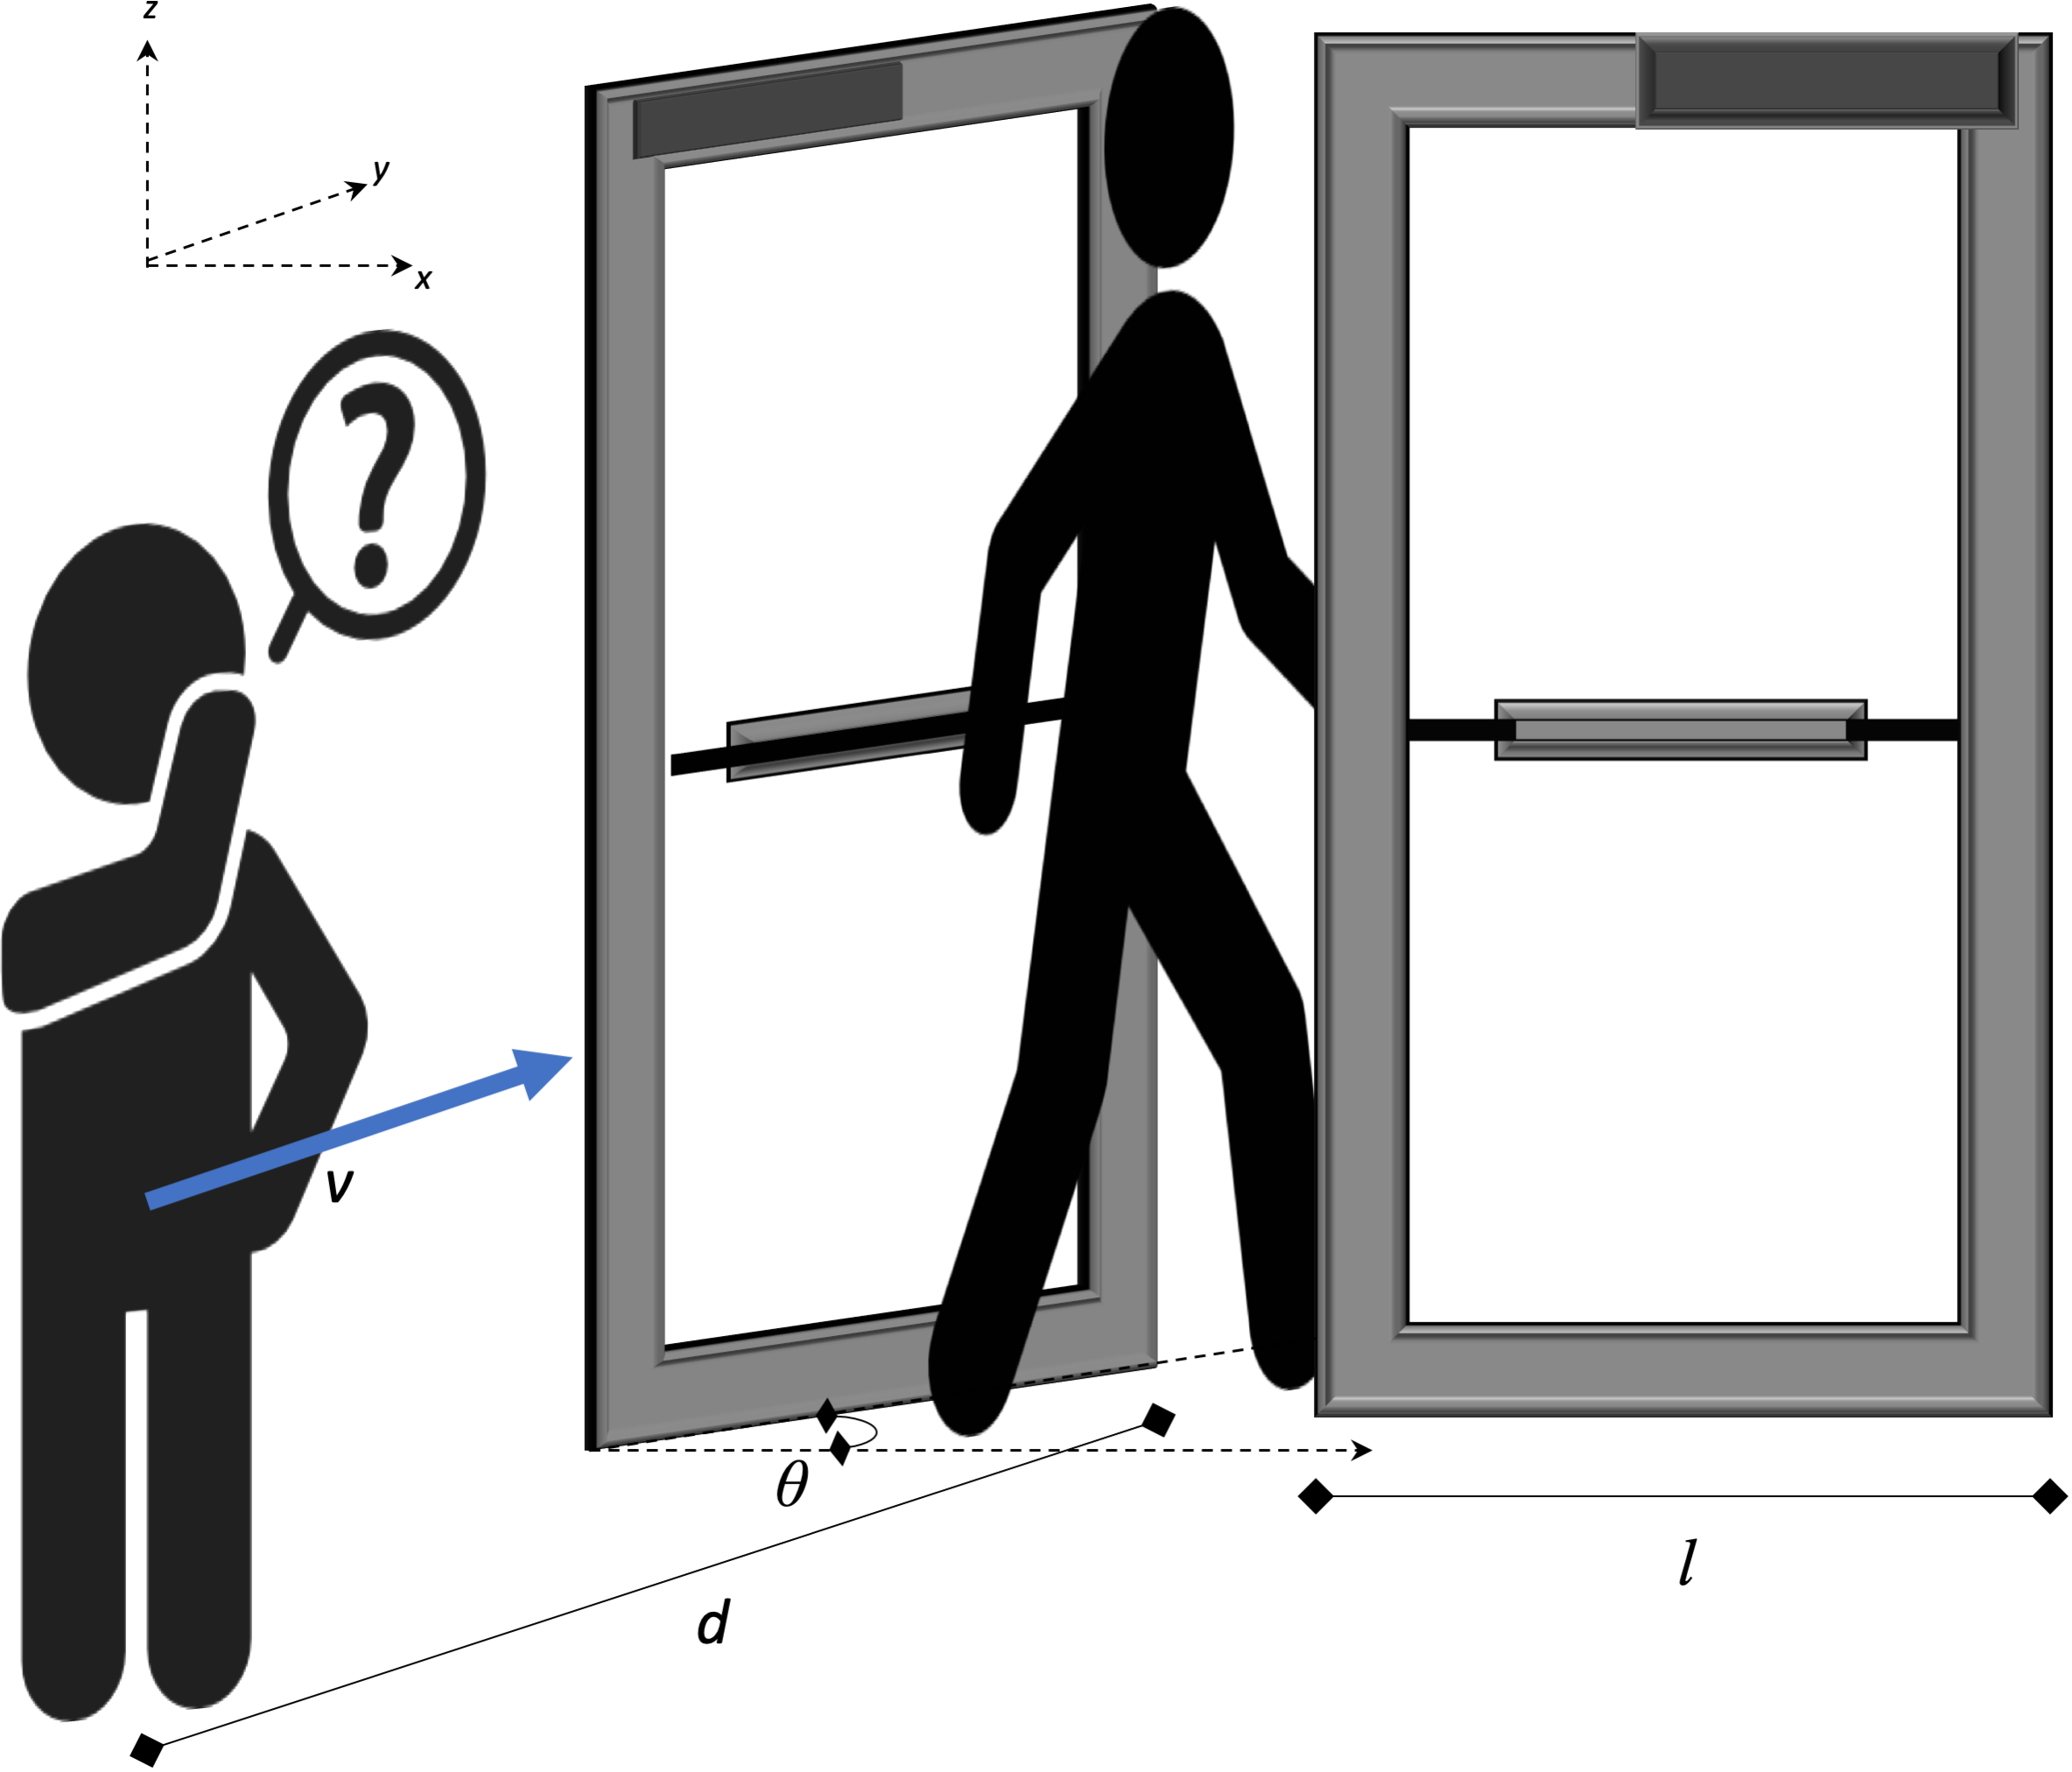
\includegraphics[width=\linewidth]{figures/Figure 1 - Schematic.png}
\caption{Simple schematic of considered problem. This event occurs immediately prior to the initializer passing through the door (thus t<0).}
\end{figure}
\section{Theoretical Model} \label{sec:Theoretical Model}
    For better understanding of the computational and experimental components of this paper, we will first establish a number of mathematical preliminaries, to better visualize the question at hand. Firstly, we will maintain the coordinate system in Figure 1, with the "x" direction being along a door (pointing from the hinges towards the knob of an unperturbed door), the (x,y) plane being that of the ground, and the "z" direction being upwards through the hinges. Any "observer" will be in reference to that person making the decision of which door to choose, and any "initializer" will be in reference to that person releasing the door, entering immediately prior to the observer. Further, let " $\vec{v}$ " be the velocity in the y-direction of the observer towards the door, let "d" be the distance between the observer and the initializer, and let "l" and "m" be the length and mass of the door, respectively. Finally, it follows that the time required for the observer to arrive at the set of doors is found by:
    \begin{eqnarray}
        v=\frac{d}{t_{0}}\Rightarrow{}t_{0}=\frac{d}{v}
    \end{eqnarray}.
    \par
    Next we must determine at what point the observer will be able to pass through the door, as surely we should not expect the observer to contort themself beyond reason. Now, the point at which a person's breadth is maximized varies (certainly on individual bases, but categorically speaking, specific groups tend to see this maximization around predominantly either the hips or the shoulders), but on average this breadth hovers around or below 40cm as found in [1]. Added to a buffer of around 10cm on each side, we will call this breadth the opening distance: $"d_{0}"\approx60cm.$ Because our door -opened to any point-, the base of the unperturbed door, and our opening distance act as sides of a triangle,in fact an isosceles triangle, we may apply the law of cosines:
    
    \begin{eqnarray}
    \begin{split}
        d_{0}^{2} & =a^{2}+b^{2}-2ab\cos(\theta_{req}) \\
        & = 2l^{2}-2l^{2}\cos(\theta_{req})
    \end{split}
    \theta_{req}=\cos^{-1}(1-\frac{d_{0}^{2}}{2l^{2}}).
    \end{eqnarray}
    Here, $\theta_{req}$ is the required angle from the x-axis in the (x,y) plane which the door must point for the observer to comfortably pass through, displayed in Figure 2(c). \par
    \begin{figure}[htp]
    \centering
    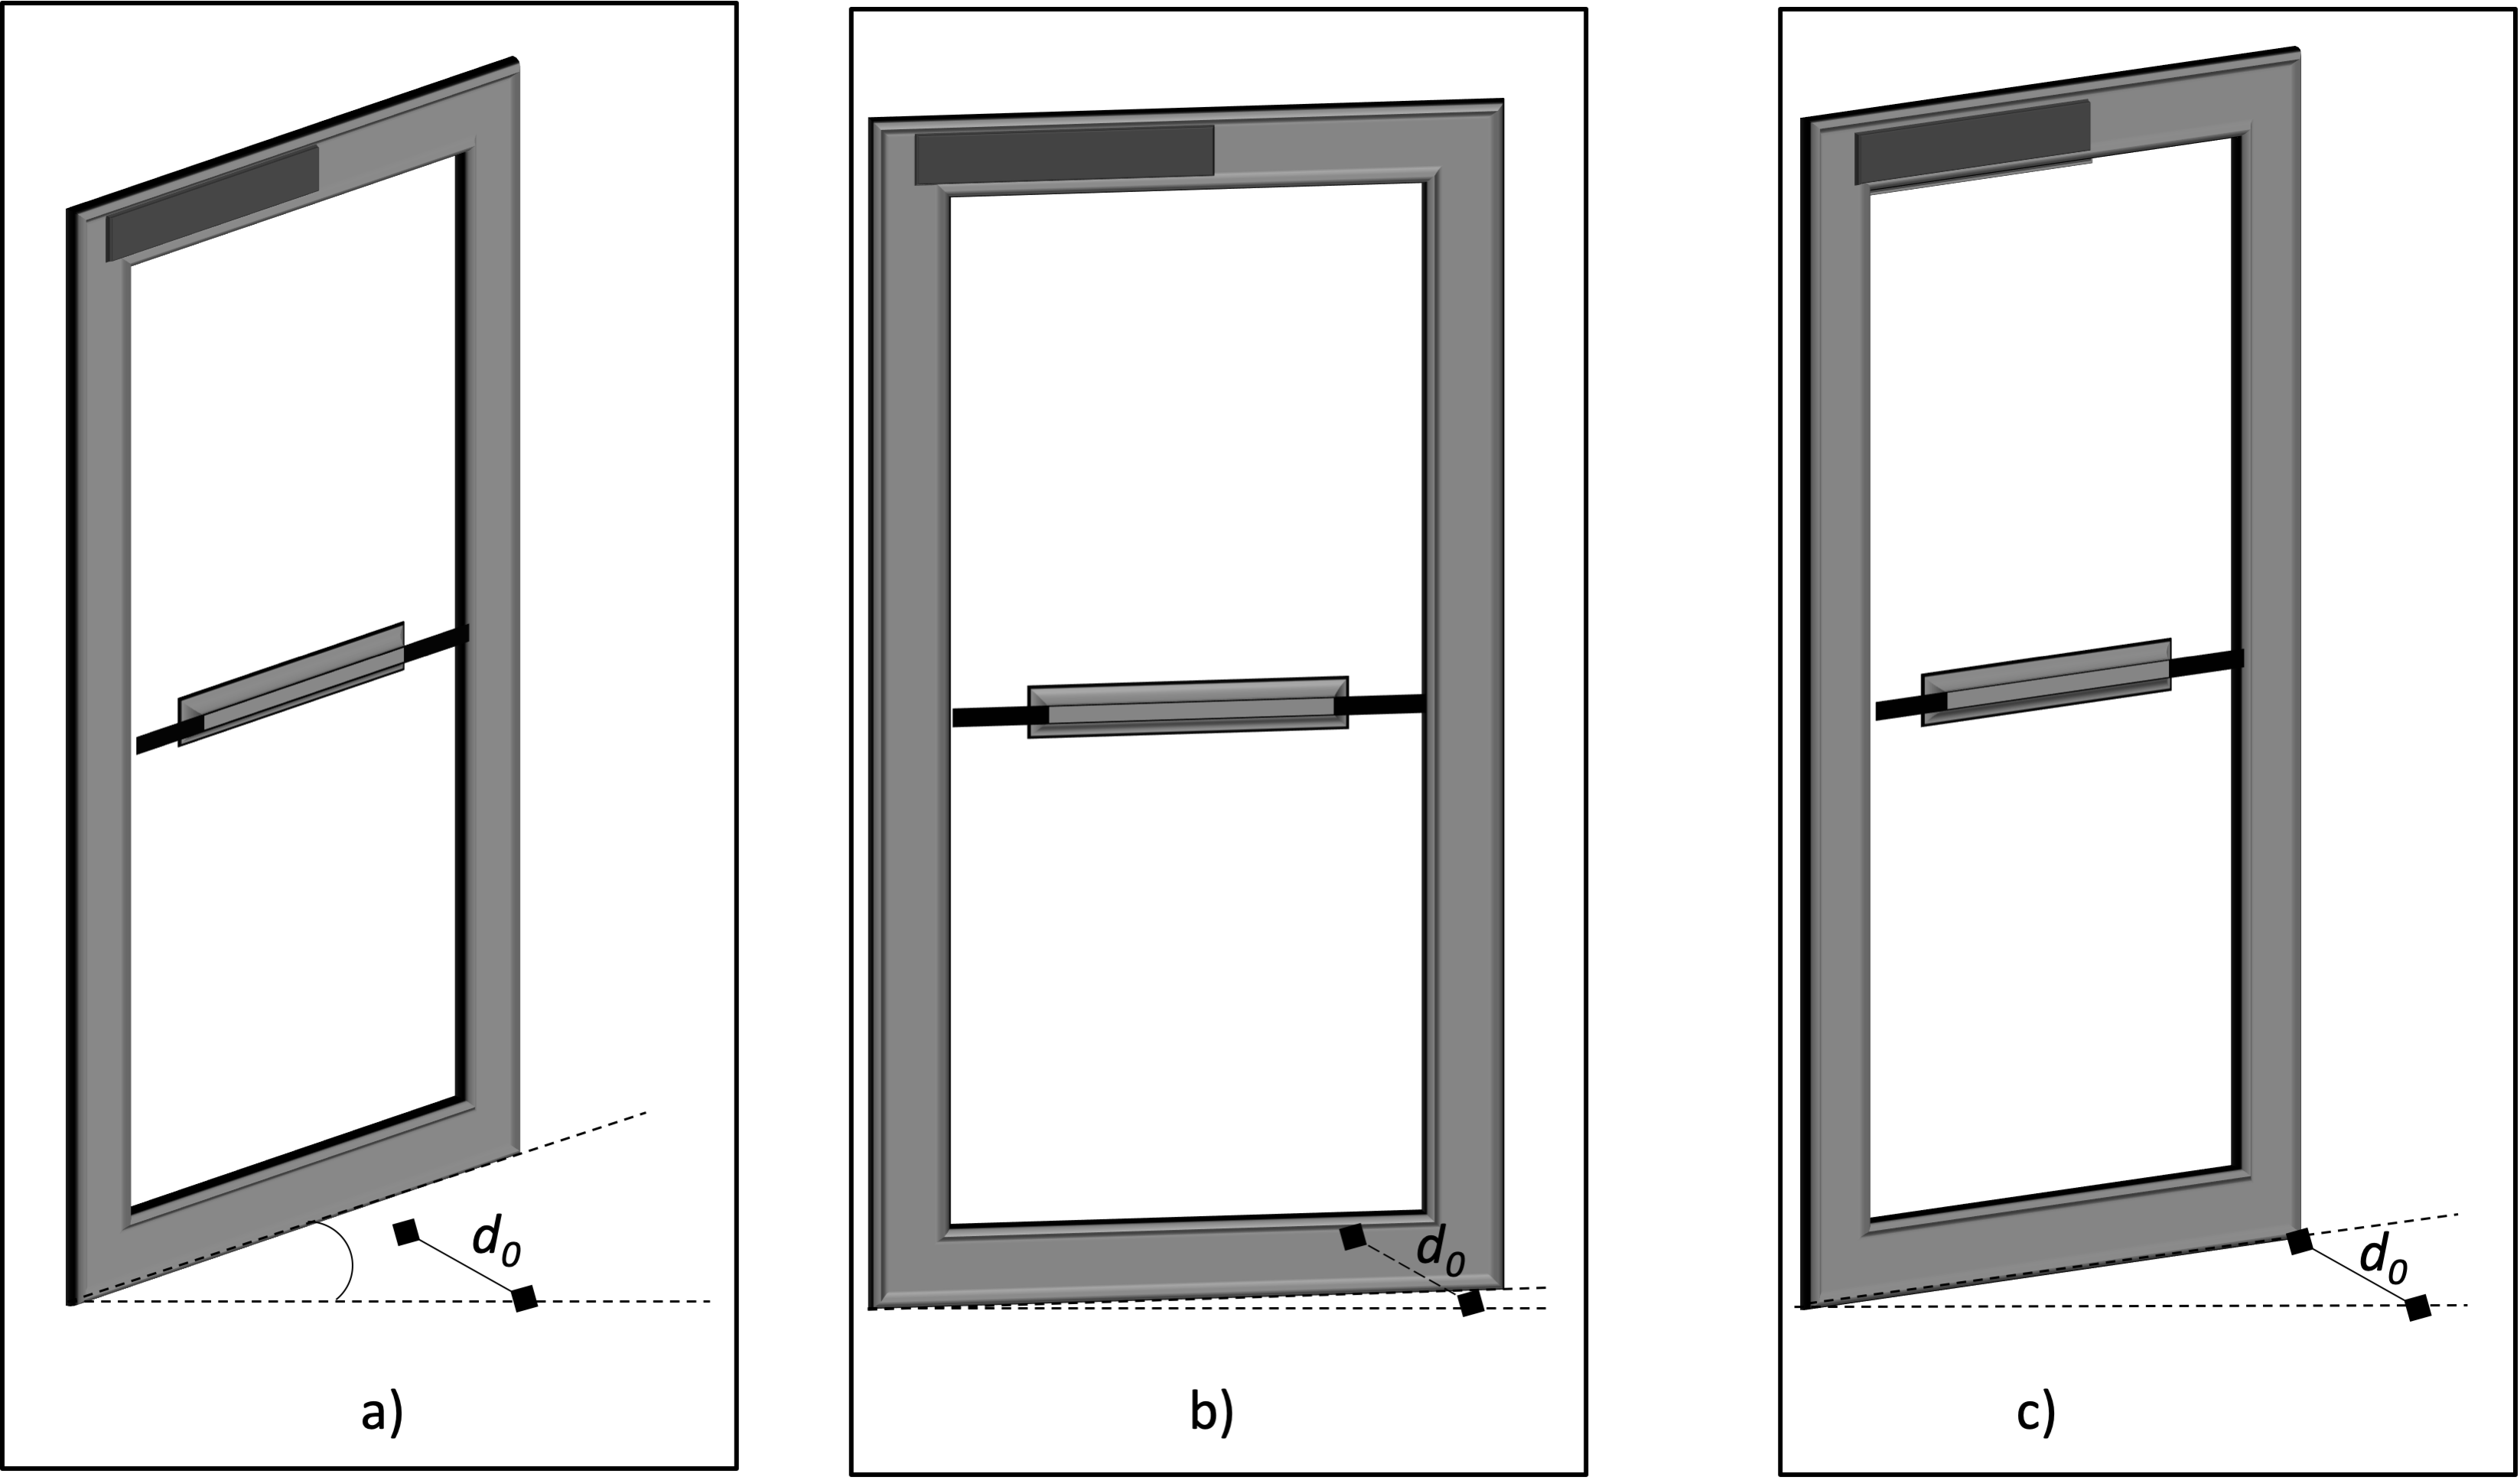
\includegraphics[width=\linewidth]{figures/Figure 2 - Angles.png}    
    \caption{A schematic showing a door opened to various angles. a) $\theta>\theta_{req}$, b) $\theta<\theta_{req}$, c) $\theta=\theta_{req}$. Also, $d_{0}$ is displayed, being the comfortable opening distance discussed.}
    \end{figure}
    We turn now to the primary question at hand, pertaining to the work required of the observer. Namely, for a force applied by the observer $\vec{F}$, perpendicular to a door pointing at some initial angle $\theta_{0}$, :
    \begin{eqnarray}
    \begin{split}
        W & =\int \Vec{F}\cdot \,\vec{dl_{\theta}}\\
        & =\int_{\theta_{0}}^{\theta_{req}} F\cdot l \,d\theta\\
        & = Fl(\theta_{req}-\theta_{0})\\
        & = \tau (\theta_{req}-\theta_{0})
    \end{split}.
    \end{eqnarray} \par
    Now, $\tau$ is some torque in the z-direction, which can be extracted from the angular impulse relation if we allow for some relatively short time $t_{impulse}$ (say 0.5s). Let the initial angular velocity of the door $\vec{\omega_{0}}$ be equal to the angular velocity of the door at time $t_{0}$ and let the final angular velocity be given by:
    \begin{eqnarray}
    \begin{split}
        \vec{\omega_{f}} & = \frac{\vec{r} \cross \vec{v}}{\norm{r}^{2}}\\
        & = \frac{v}{l},
    \end{split}
    \end{eqnarray}
    the former of which will be derived for the cases in the following subsections. Note, then that the angular momenta are:
    \begin{eqnarray}
    \begin{split}
        L_{0}=I\vec{\omega_{0}}=I\omega_{0,z}, \text{ and }  L_{f}=I\vec{\omega_{f}}=\frac{Iv}{l},
    \end{split}
    \end{eqnarray}
    and thus,
    \begin{eqnarray}
    \begin{split}
        \Delta L & = L_{f}-L_{0} = \frac{Iv}{l}-I\omega_{0,z}=\\
        & = I(\frac{v}{l}-\omega_{0,z})=\tau t_{impulse},
    \end{split}\\
    \begin{split}
        \tau & =\frac{I}{t_{impulse}}(\frac{v}{l}-\omega_{0,z}).
    \end{split}
    \end{eqnarray}\par
    Further, if we consider the door to have a uniform mass distribution $\rho=\frac{m}{l}$ and to be rotating about the hinges, we have that
    \begin{eqnarray}
    \begin{split}
        I & =\int_{0}^{l} \rho r^{2} \,dr = \frac{1}{3} \rho r^{3} |_{0}^{l}=\frac{1}{3}\frac{m}{l}l^{3}\\
        & = \frac{1}{3}ml^{2}.
    \end{split}
    \end{eqnarray}
    Thereby, we can substitute equations (8) and (9) into equation (4) to find:
    \begin{eqnarray}
    \begin{split}
        W & =\frac{1}{3}\frac{ml^{2}}{t_{impulse}} (\theta_{req}-\theta_{0}) (\frac{v}{l}-\omega_{0,z}).
    \end{split}
    \end{eqnarray}
    Note that the units are consistent with units of work. Also note that, as expected, if $\theta_{0}>\theta_{req}$ then the work is negative, being that any further energy exerted by the observer would not make it any easier to comfortably fit through the door. Finally, note that the work needed to open the unopened door to the required angle (i.e. when both $\omega_{0,z}$ and $\theta_{0}$ are identically 0) is given by:
    \begin{eqnarray}
    \begin{split}
        W & = \frac{1}{3}\frac{mlv}{t_{impulse}}.
    \end{split}
    \end{eqnarray}\par
    We will next consider Undamped, as well as Critically and Overdamped manual door closers, and in specific, derive the $\omega_{0,z}$ defined in this problem for each case. We will additionally do this for an Underdamped case, in a similar problem involving a double hinged door.
    \subsection{Undamped Case}
    For each of these cases, one might find it helpful to envision a common mass-spring system, or simple pendulum; and particularly, review of of references [2] and [3] could prove useful. Here, at $t=0$ we have that the door has been released by the initializer, and the manual door closer has begun to move the door back towards it's equilibrium position. Let the angular acceleration describing the door's motion be $a_{\theta}=l\ddot\theta$, and let the torque of the manual door mover be $\tau_{m}=-\kappa\theta$, where $\kappa$ is some torsion coefficient. The force on the door can thus be found:
    \begin{eqnarray}
    \begin{split}
        \tau & = \vec F \cdot \vec r = F(\theta)l = -\kappa \theta,
    \end{split}
    \begin{split}
        F(\theta) & = -\frac{\kappa}{l}\theta,
    \end{split}
    \end{eqnarray}
    which will be equivalent to the sum of all forces acting on the door, $\sum F$, while $t\in[0,t_{0}]$.\par
    We then have, by Newton's second law:
    \begin{eqnarray}
    \begin{split}
        ma_{\theta}=F(\theta)\\
        ml\ddot\theta = -\frac{\kappa}{l}\theta\\
        ml\ddot\theta+\frac{\kappa}{l}\theta=0\\
        \ddot\theta + \frac{\kappa}{ml^{2}}\theta=0.
    \end{split}
    \end{eqnarray}
    To avoid confusion with the above formalism, we will define the constant $c^{2}\equiv\frac{\kappa}{ml^{2}}$ (instead of the commonly used $\omega_{0}^{2}$). We then have that (13) is a second order ordinary differential equation with solution:
    \begin{eqnarray}
    \begin{split}
        \theta(t)=A\cos(ct+\phi),
    \end{split}
    \end{eqnarray}
    where A and $\phi$ are constants.\par
    To determine these constants, we must have the angle at which the initializer releases the door and at what angular velocity they release it at, call them $\theta(0)\equiv\theta_{i}$ and $\dot\theta(0)\equiv\dot\theta_{i}$, respectively. We can then use (14) and the fact that
    \begin{eqnarray}
    \begin{split}
        \dot\theta(t)=\frac{d}{dt}A\cos(ct+\phi)=-Ac\sin(ct+\phi)
    \end{split}
    \end{eqnarray}
    to see that
    \begin{eqnarray}
    \begin{split}
        \cos^{2}(\phi) = \frac{\theta_{i}^{2}}{A^{2}} \text{ and }
        \sin^{2}(\phi)=\frac{\dot\theta_{i}^{2}}{c^{2}A^{2}}
    \end{split}\\
    \end{eqnarray}
    so that
    \begin{eqnarray}
    \begin{split}
        A^{2}=\theta_{i}^{2}+\frac{\dot\theta_{i}^{2}}{c^{2}}, \text{ or }
        A=\sqrt{\theta_{i}^{2}+\frac{\dot\theta_{i}^{2}}{c^{2}}},
    \end{split}
    \end{eqnarray}
    and using (17) in (14), we have that 
    \begin{eqnarray}
    \begin{split}
        \phi=\frac{\theta_{i}}{\sqrt{\theta_{i}^{2}+\frac{\dot\theta_{i}^{2}}{c^{2}}}}
    \end{split}.
    \end{eqnarray}\par
    Finally, from (15), we can find the angular velocity for our considered problem:
    \begin{eqnarray}
    \begin{split}
        \omega_{0,z} & = \dot\theta(t_{0})=-Ac\sin (ct_{0}+\phi)
    \end{split}.
    \end{eqnarray}
    and equation (9) becomes
    \begin{eqnarray}
    \begin{split}
        W & =\frac{1}{3}\frac{ml^{2}}{t_{impulse}}(\theta_{req}-\theta_{0}) (\frac{v}{l}+Ac\sin(ct_{0}+\phi)),
    \end{split}
    \end{eqnarray}
    with each of the constants as previously defined. \\
    \subsection{Damped Cases}
    Though the undamped case is certainly interesting, it hardly can be applied generally to the situation at hand. In fact, the undamped case would be better suited for something like a door which closes using a spring (similar to the way a mouse/rat trap might close), rather than the typical manual closer found commonly throughout everyday life. It is thus necessary to consider the case of dampened manual door closers, and their impact on our problem.\par
    We start similarly that of the undamped case, by calling the same $a_{\theta}$ and $F(\theta)$, however this time, the sum of the forces acting on the door will have an additional angular-velocity-limiting factor:
    \begin{eqnarray}
    \begin{split}
        \sum F & = \alpha\vec v_{\tan,door} + F(\theta) = -bl\dot\theta-\frac{\kappa}{l}\theta
    \end{split}.
    \end{eqnarray}
    Equation (12) then becomes
    \begin{eqnarray}
    \begin{split}
        \ddot\theta+\frac{b}{m}\dot\theta+\frac{\kappa}{ml^{2}}\theta=0
    \end{split},
    \end{eqnarray}
    and if we allow again the constant $c^{2}\equiv\frac{\kappa}{ml^{2}}$ and replace $\frac{b}{m}\equiv2\beta$, the corresponding general solution of (23) is
    \begin{eqnarray}
    \begin{split}
        \theta(t)=e^{-\beta t}(A_{1}e^{\sqrt{\beta^{2}-c^{2}}t}+A_{2}e^{-\sqrt{\beta^{2}-c^{2}}t})
    \end{split}.
    \end{eqnarray} \par
    We thus have three cases, as per usual:
    $\beta^{2}>c^{2}$, called overdamping, in which case the square roots are real and the corresponding equation is a decaying exponential; $\beta^{2}=c^{2}$, called critically damping, which also results in a decaying exponential, though it has no buffer and goes to zero much faster than the overdamped case; and $\beta^{2}<c^{2}$, called underdamping, in which case the square roots are imaginary, and the resulting equation resembles that of a cosine function. Note that the underdamped case, if the door is single hinged, will act similarly to that of the undamped case (in that they both are resembling cosine functions), though with a decaying factor "tacked on". We will develop this resemblance further in our discussion of the double hinged door, as well as determine the $\omega_{0,z}$ for each case.\\
    \subsubsection{Overdamped and Critically-damped Cases}
    For the Overdamped case, we begin with defining a $c_{0}=\sqrt{\beta^{2}-c^{2}}$, so that (23) will become
    \begin{eqnarray}
    \begin{split}
        \theta(t)=e^{-\beta t}(A_{1}e^{c_{0}t}+A_{2}e^{-c_{0}t})
    \end{split}.
    \end{eqnarray}
    Now we may find the angular velocity at time $t_{0}$:
    \begin{eqnarray}
    \begin{split}
        \omega_{0,z} & =\dot\theta(t_{0})\\
        & =(A_{1}(c_{0}t+\beta)e^{2c_{0}t}+A_{2}(c_{0}-\beta))e^{-t(c_{0}-\beta)}.
    \end{split}
    \end{eqnarray}
    Here, we have:
    \begin{eqnarray}
    \begin{split}
        \theta(0)=\theta_{i}=A_{1}+A_{2}, \text{ as well as }\\ \dot\theta(0)=\dot\theta_{i}=A_{1}\beta+A_{2}(c_{0}-\beta),
    \end{split}
    \end{eqnarray}
    and with some algebraic manipulation, we find
    \begin{eqnarray}
    \begin{split}
        A_{2}=\frac{\beta\theta_{i}-\dot\theta_{i}}{2\beta-c_{0}}, \text{ and }
        A_{1}=\theta_{i}-\frac{\beta\theta_{i}-\dot\theta_{i}}{2\beta-c_{0}}
    \end{split}.
    \end{eqnarray}
    It would then suffice to insert (26) into (9) to determine a solution to our problem.\par
    Next, for the critically damped case, we have that our $c_{0}^{2}=\beta^{2}$. Here, the solution to (23) is not (24), but rather the general solution for a repeated root:
    \begin{eqnarray}
    \begin{split}
        \theta(t)=e^{-\beta t}(A+Bt)
    \end{split},
    \end{eqnarray}
    and our angular velocity at time $t_{0}$ is
    \begin{eqnarray}
    \begin{split}
        \omega_{0,z}=\dot\theta(t_{0})=e^{-\beta t_{0}}(B(1-\beta t_{0})-A\beta)
    \end{split}.
    \end{eqnarray}
    We can use our initial conditions to find the constants A and B:
    \begin{eqnarray}
    \begin{split}
        \theta(0)=\theta_{i}=A, \text{ and }\\
        \dot\theta(0)=\dot\theta_{i}=B-A\beta, \text{ or } B=\dot\theta_{i}+\theta_{i}\beta,
    \end{split}
    \end{eqnarray}
    and similarly to the overdamped case, insert (30) into (9) to gather a solution to our problem. 
    \subsubsection{Underdamped Case (double-hinged doors)}
	For the Under-damped Case, we define $c_{0}=\sqrt{\beta^{2}-c^{2}}$, as $\beta^{2}-c^{2}<0$, then we can rewrite $c_{0}=\sqrt{c^2-\beta^{2}}i$. So that (24) will become
    \begin{eqnarray}
    \begin{split}
      \theta(t)=e^{-\beta t}(A_{1}e^{c_{0}t}+A_{2}e^{-c_{0}t})
    \end{split}
    \end{eqnarray}
    Now we find the angular velocity at time t0:\begin{eqnarray}
    \begin{split}
        \omega_{0,z} & =\dot\theta(t_{0})\\
        & =(A_{1}(c_{0}t+\beta)e^{2c_{0}t}+A_{2}(c_{0}-\beta))e^{-t(c_{0}-\beta)}.
    \end{split}
    \end{eqnarray}
    Here, we have :
      \begin{eqnarray}
    \begin{split}
        \theta(0)=\theta_{i}=A_{1}+A_{2}, \text{ as well as }\\ \dot\theta(0)=\dot\theta_{i}=A_{1}\beta+A_{2}(c_{0}-\beta),
    \end{split}
    \end{eqnarray}  and with some algebraic manipulation, we find
    
    \begin{eqnarray}
    \begin{split}
        A_{2}=\frac{\beta\theta_{i}-\dot\theta_{i}}{2\beta-c_{0}}, \text{ and }
        A_{1}=\theta_{i}-\frac{\beta\theta_{i}-\dot\theta_{i}}{2\beta-c_{0}}
    \end{split}.
    \end{eqnarray}
      It would then suffice to insert (34) into (9) to determine a solution to our problem.\par

    

\section{Description of Numerical/Experimental Procedures} \label{sec:Description of Numerical/Experimental Procedures}
    \subsection{Numerical/Computational procedure}
            \par{} The main algorithm behind the computational model comes from a Fourth Order Runge-Kutta Integrator. Consider some differential equation:
        \begin{equation}
            \frac{dy(t)}{dt} = f(y(t),t)
        \end{equation}
            One can numerically approximate the equation of the line by using ghost steps at very small steps $h$ across the function $y(t)$. The equations for these ghost steps are given as the following:
        \begin{align} 
            & {k_1} = f({y^*}({t_0}),{t_0})  \\  
            & {k_2} = f\left( {{y^*}({t_0}) + {k_1}{h \over 2},{t_0} + {h \over 2}} \right)  \\
            & {k_3} = f\left( {{y^*}({t_0}) + {k_2}{h \over 2},{t_0} + {h \over 2}} \right)  \\  
            & {k_4} = f\left( {{y^*}({t_0}) + {k_3}h,{t_0} + h} \right)
        \end{align}
        Then one can take the weighted sum of the the ghost points to give that the next step along the line is the following:
        \begin{equation}
            {y^*}(t_0 + h) = {y^*}(t) + h\frac{k_1 + 2k_2 + 2k_3 + k_4}{6}
        \end{equation}
        \par{} Here, we use this form of integration technique for the computational accuracy of the algorithm and the flexibility of the integrator. All one needs is the differential equation of motion and then a computer can do the heavy lifting. We thus consider the differential equation of motion described in the theoretical model:
        \begin{eqnarray}
            \begin{split}
                \ddot\theta+\frac{b}{m}\dot\theta+\frac{\kappa}{ml^{2}}\theta=0
            \end{split}.
        \end{eqnarray}
    \subsection{Experimental procedure}
    There are many factors to account for in this project which would be rather difficult to measure experimentally. In particular, measuring something like the torsion coefficient would be rather difficult, and even seemingly simple measurements such as the mass of a door prove to be rather tedious to obtain (especially considering administrative constraints). We then have done our best with what we have (and a few extra tools).\par
    Firstly, we found a door which had a manual closer; initially, our intention was to use the doors in our Interdisciplinary Sciences building. However, the precautionary measures against the spread of COVID-19 has forced us to move a bit closer to home, in fact we chose a porch screen door which leads to the back yard of Mr. Hart.\par
    Next, we wanted some method by which to measure the net force on the door. Luckily, this can be accomplished by means of a door pressure gauge, which is a small metal rod attached to some springs within a chamber, and when pressed against a door, tick marks on the bar can be read out as being the force exerted by the door on the gauge. Obviously, we placed our pressure gauge where one might typically press their hand against a door (much closer to the "handle" than the hinges), and made our all our measurements from the same spot on the door. We first measure the force as we open the door until we read a maximum angle (where we see the force spike), then start to recede and note any changes in the force (due to damping effects).\par
    Finally, we needed a way to measure angular acceleration and angular velocity of the door. We first placed a large piece of paper below the door (ensuring the door was not scraping against it, to avoid an additional frictional force), with lines corresponding to certain angles: 125°(the maximum to which the door could open), 90°, 60°, 45°, 36.9°, 30°, 15°, and 7° drawn onto it. We then time the door closing on a stopwatch and lap every time it passes a line, then plot 5 sets of these measurements and fit a curve to the data.\par
    From these we find some interesting results, in which we can compare the net force on the door to the door's motion.
\section{Data Analyses} \label{sec:Data Analyses}
    \subsection{Computational Analysis}
        We then choose a damping coefficient ($b=0.4$) and a torsion coefficient ($\kappa = .1$) and then run the RK4 simulator for the experimentally measured angles ($125, 90, 60, 45, 30, 15, 0$). Using the numpy's real Fast Fourier Transform (numpy.fft.rfft()). We find that the $c_0$ for each initial angle: 
        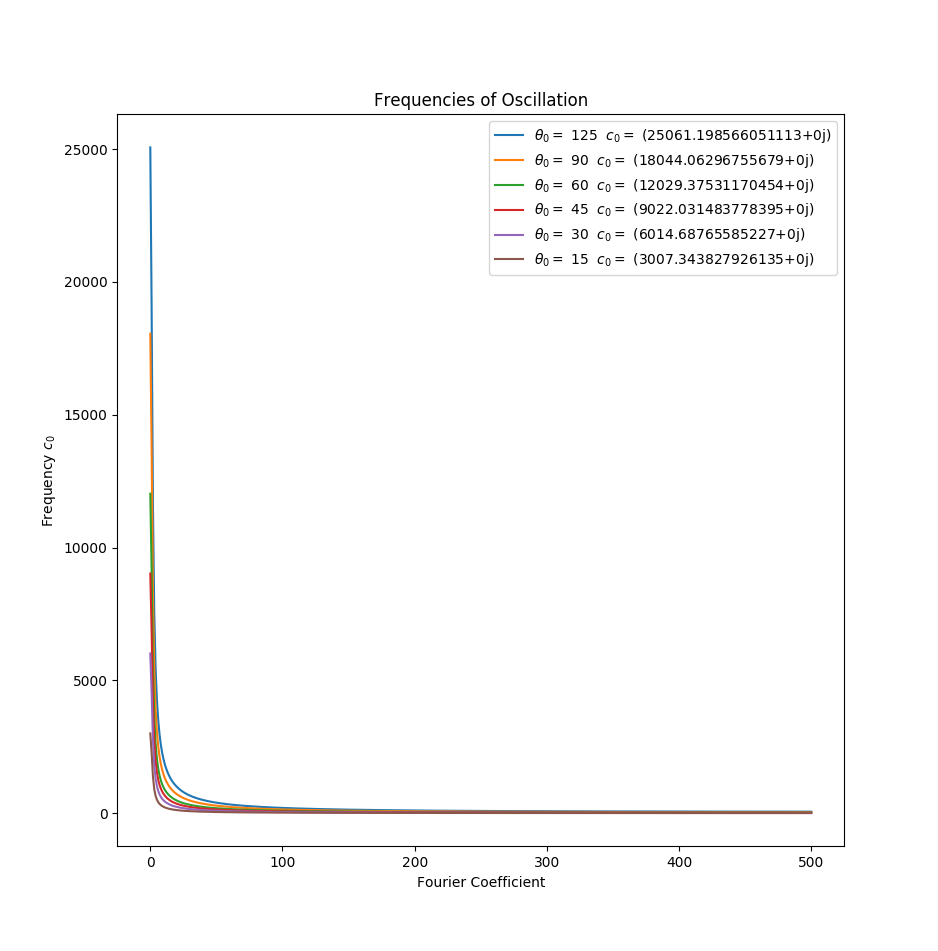
\includegraphics[width=\linewidth]{figures/Figure 3 - Angular Frequancies .png}
        Then we can find that the angular phase portrait for each initial angle is given as: 
        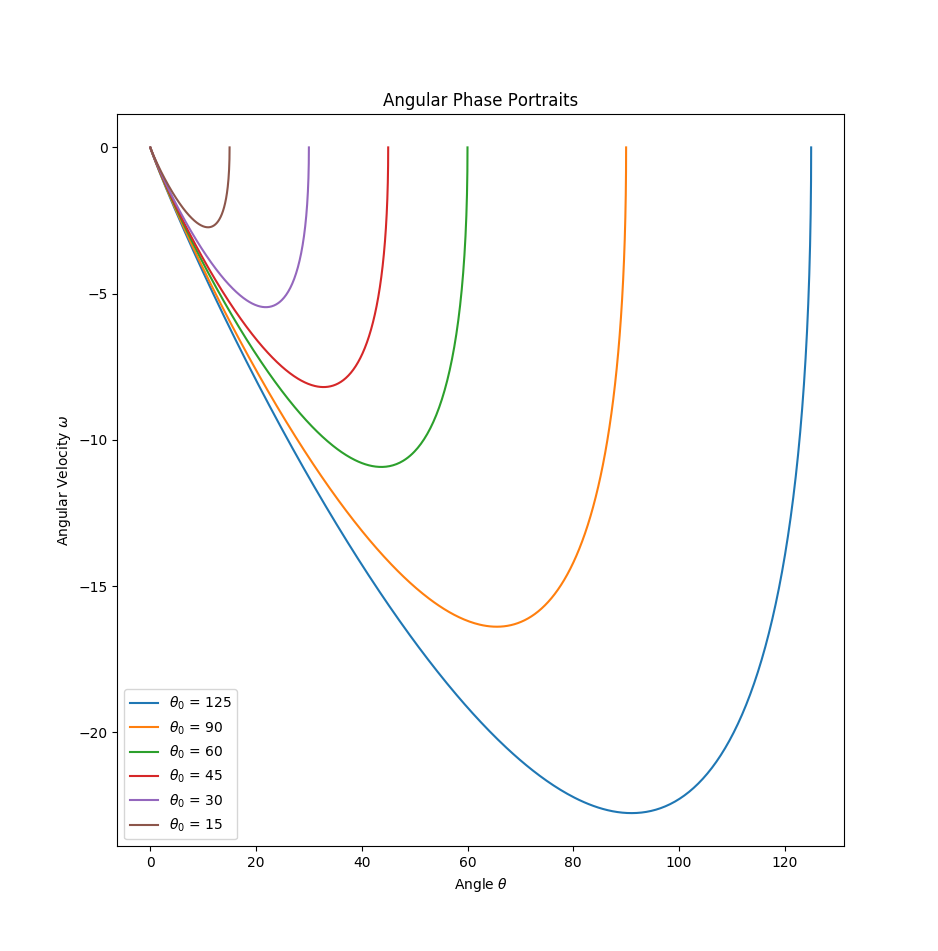
\includegraphics[width=\linewidth]{figures/Figure 4 - Angular Phase Portrait.png}
    \subsection{Experimental Analysis}
        For the measurement of the force, we (unfortunately) were only able to measure in pounds, so later we convert to Newtons. The tick marks were at each whole pound, so any decimal is an estimation. The door showed having a consistent 2.0lb of force (pounds are force in imperial units, luckily, and fun fact, the "slug" is the imperial unit of mass) when opened as described in the procedure above. When receding back to zero, however, we note that in-between the 60° and 45°markings, the force dropped from 2.0lb to roughly 1.2lb. We continued to read this measurement until the door hit something like a "release" in between 15° and 7° (in fact, it was after noticing this that we chose to include the angle measurement at 7°), where the reading evidently jumped back up to 1.6lb.\par
        For the angle versus time measurements, we have included all our recorded data as seen in Table I. Further we have used MATLAB to plot the angle versus time scatter plot in Figures 3 (a), and the angular velocity and angular acceleration plots Figure 3 (b)-(c).
        \begin{center}
            \begin{table}
            \begin{tabular}{||c || c c c c c||} 
            \hline
            Angle range & Trial 1 & Trial 2 & Trial 3 & Trial 4 & Trial 5\\ [0.5ex] 
            \hline\hline
             125°-90° & 1.48s &  1.42s & 1.48s & 1.39s & 1.5s \\ 
            \hline
            90°-60° & 1.93s & 1.95s & 2.09s & 1.90s & 1.89s \\
            \hline
            60°-45° & 5.58s & 5.32s & 5.92s & 5.30s & 5.41s \\
            \hline
             45°-37° & 8.15s & 6.90s & 7.60s & 6.73s & 6.83s \\
            \hline
            37°-30° & 12.75s & 12.41s & 11.76s & 11.14s & 11.49s \\ 
            \hline
            30°-15° & 21.68s & 19.61 & 19.03s & 19.50s & 20.12s\\
            \hline
            15°-7° & 26.37s & 25.42 & 24.56s & 24.09s & 25.05s\\ [1ex] 
            \hline
            \end{tabular}
            \caption{Data collected from a screen door with manual closer}
            \label{table:1}
            \end{table}
        \end{center}
        \begin{figure}[htbp]
        \centering
        \subfloat[Angle vs. Time plot]{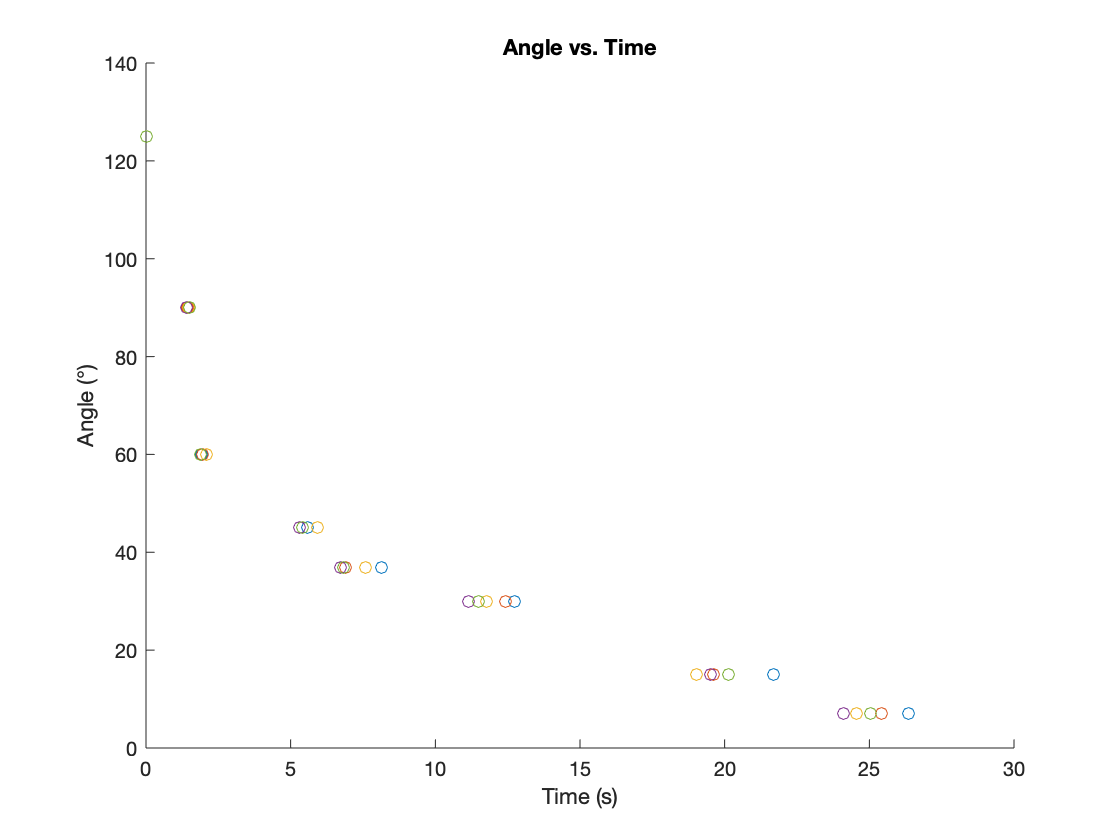
\includegraphics[width=\linewidth]{figures/Figure 3a - Angle vs Time.png}}\\
        \subfloat[Angular Velocity vs. Time plot]{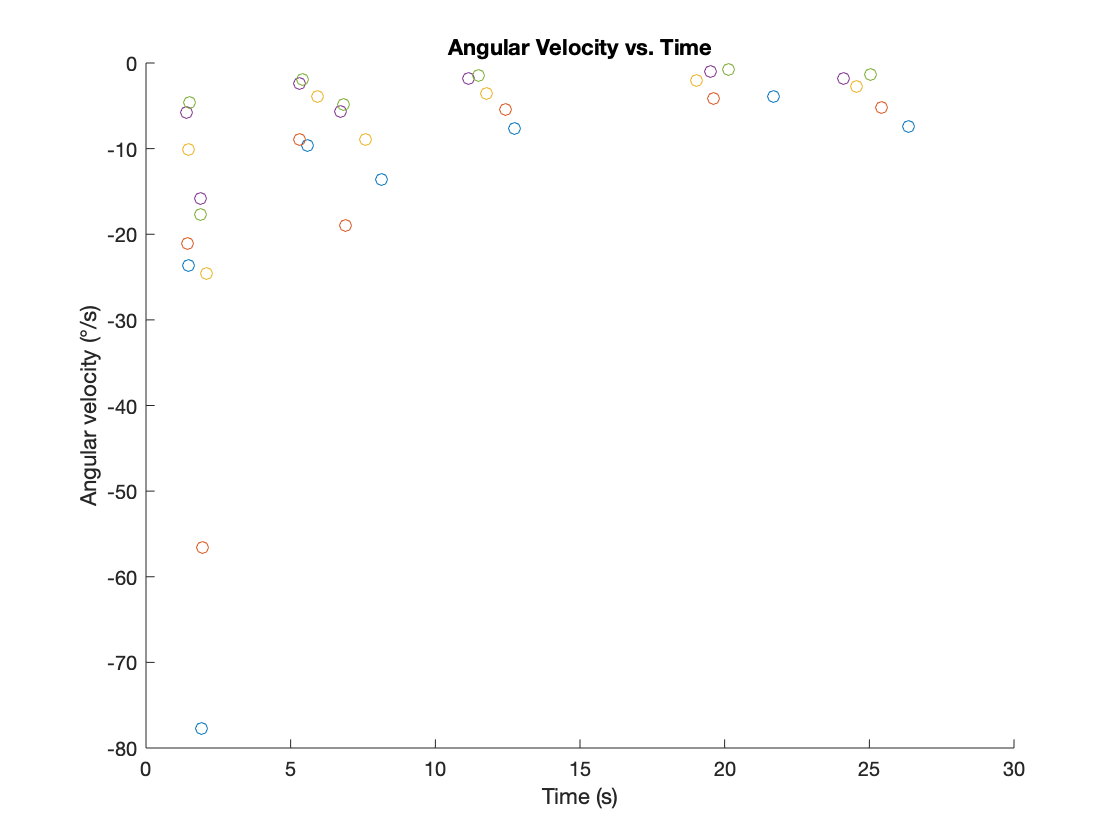
\includegraphics[width=\linewidth]{figures/Figure 3b - Angular Velocity vs Time.png}}\\
        \subfloat[Angular Acceleration vs. Time plot]{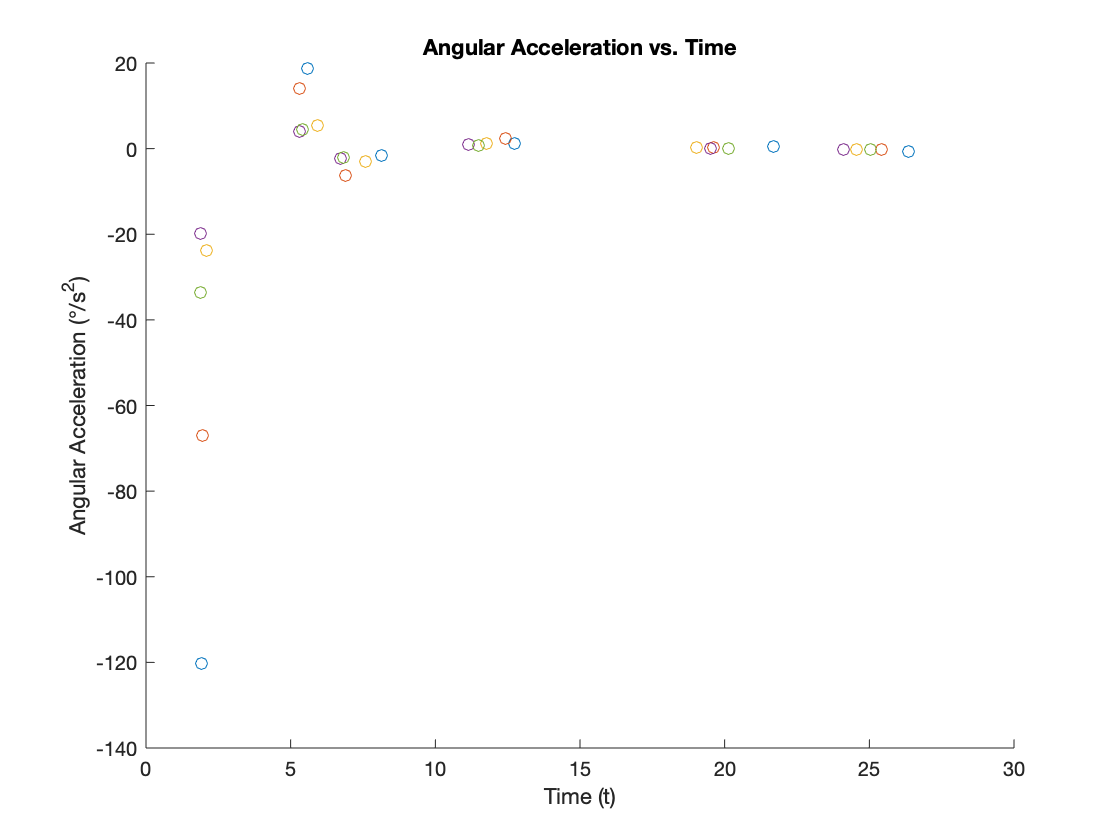
\includegraphics[width=\linewidth]{figures/Figure 3c - Angular Acceleration vs Time.png}}
        \caption{MATLAB plots for experimental results}
        \end{figure}\par
        Notice that in the Figure 3a , the first three points resemble that of a negative quadratic function of time ($-t^{2}$), but then the rest of the points appear to correlate more with an negative exponential function of time ($e^-{t}$) as in our overdamped and critically damped cases. We note that from our formalism, an undamped case for the function of the angle with time would resemble a cosine funtion, and when approximated to the second degree Taylor polynomial, this cosine function is in fact a dominated by a negative quadratic. Thus we would expect that for those first three points (roughly), our manual closer provided no damping, and after the third point the closer began to apply some retarding force. Both of these are fully consistent with the force measurements which we have taken. \par
        Further, note that towards the final points on Figure 3 (b) and (c) that the angular velocity and angular accelerations decrease (with respect to an opening frame of reference). As we have previously mentioned, the door seemed to have some release mechanism towards the smallest angles where, the force seemed to spike back up. These changes in the angular velocities and angular accelerations (though minuscule) show this phenomenon quite nicely.
        
\section{Conclusion} \label{sec:Conclusion}
To conclude, we will discuss the scope of this work in brief. We have developed a number of mathematical formalisms to help solve the problem described in the introduction, and have used these to describe the motion of a door experimentally, as well as to develop computational systems to model events under ideal conditions. We have only to answer the question of which door to take, which after reading the first two pages is nearly trivial.  Whichever of equations (9) or (10) is lesser for the situation's specific case of manual door closer will correspond to their choosing the open or closed door respective, to have the easiest time passing through (or the converse to get a better workout).\par
The only caveat is that not all door dampeners work with a single modality, such as the screen door we have used in our experiments. Though the formalism is evidently descriptive of each type of dampening, it is obvious that some door dampeners, such as the one considered here, also apply their effects as some function of the angle (in this case, no effect for ~125°-45° and ~7°-0°, and some critical or overdamped effect for ~45°-7°). These will obviously vary by make and model, and a discussion on which is best engineering practice may certainly follow from this paper.
\section*{Acknowledgements} \label{sec:acknowledgements}
    I would like to thank Dr. Shi for approving this project, as it has been a question I have held for a long time though likely never would have developed without some incentive. Additionally, we very much appreciate the criticisms and suggestions made by our peer editors: Christopher Taylor, Yasif Rahman, and Angel Bojorge. Finally, we would like to thank the physics department here at USF, for fostering knowledge and challenging students to learn and achieve (and especially for the experience in utilization of LaTeX for future work in the STEM fields).

\begin{thebibliography}{4}
\bibitem{NON}
NASA,
\textit{Anthropometric source book. Volume 1: Anthropometry for designers}
(NASA tech docs, 1978).

\bibitem{Marion Thornton}
Marion-Thornton,
\textit{Classical Dynamics}
(Saunders College Pub, Fort Worth, 1995).

\bibitem{Taylor}
John R. Taylor,
\textit{Classical Mechanics}
(University Science Books, Sausalito, Calif. 2005).

%\bibitem{Jackson-CE}
%J. D. Jackson,
%\textit{Classical Electrodynamics}
%(John Wiley \& Sons, Danvers, 1999).
\end{thebibliography}

%\appendix*
%\section{Appendix} \label{sec:appendix}
    

\end{document}
